\section{Joystick Control}\insertloftspace
\setcounter{figure}{0}\setcounter{table}{0}

\subsection{Principle}

The initial request of our customer was a remote-controlled arm. This was the easiest and fastest solution to implement. Mr. Kedziora also wanted to avoid using artificial intelligence in order not to lengthen the prototype manufacturing time. Despite our fears about the difficulties that this type of order can pose, he really insisted that we use this method, which is the first one that we have put in place.

\bigbreak
In this configuration, a camera, fixed on the arm at the level of the hand, allows the user to have a video return. An Xbox controller in our case is used to control the arm. The commands sent by the user are done in the camera's frame.
\begin{figure}[H]
    \begin{subfigure}{.5\linewidth}
        \centering
        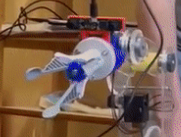
\includegraphics[width=0.95\textwidth]{Images/Section07/camera.png}
        \caption{Position}
        \label{fig:CameraRobot}
    \end{subfigure}%
    \begin{subfigure}{.5\linewidth}
        \centering
        \includegraphics[width=0.95\textwidth]{Images/Section07/camera\_view.png}
        \caption{View}
        \label{fig:CameraView}
    \end{subfigure}\\[1ex]
    \caption{Camera}
    \label{fig:Camera}
\end{figure}
\FloatBarrier

\bigbreak
The control of the three axes in the camera frame is done with the two joysticks on the controller. The left joystick allows to move according to the plane (x,y) of the camera (see \ref{fig:kinematicsSchema} and the right joystick manages the depth. This movement is then transformed into a command to move along the desired axis. Some features listed below have also been added to the buttons to facilitate the work of the user and the proper functioning of the arm.
\begin{itemize}[noitemsep]
    \item authorize the movement: button A
    \item prohibit the movement: button B
    \item return to zero position : button X
    \item return to deposit position : button Y
\end{itemize}

\begin{figure}[ht]
    \centering
    \includegraphics[width=0.6\textwidth]{Images/Section07/xbox\_controller.png}
    \caption{Xbox Controller}
    \label{fig:XboxController}
\end{figure}
\FloatBarrier

\bigbreak
As explained in the previous section, the inverse kinematics calculates the necessary angles for a given position in the base frame \{s\}. However, it seemed more natural to us to make the user work in the camera reference frame \{c\} and then to change the reference frame. For this, we reused the modern robotics library. In the same way that we can calculate the transformation matrix between the base and the end effector from the position of the links, we can calculate the one between the base and the camera. 
\begin{center}
    $T_{sc} =\displaystyle \prod_{n=1}^4e^{[S_i]\theta_i}M_c$
\end{center}

\bigbreak
Then the relation between the position in the reference frame and the position in the reference frame is the following:
\begin{center}
    $p_s = T_{sc}p_c$
\end{center}

\bigbreak
Attention, $T_{sc}$ being a 4x4 matrix, $p_s$ and $p_c$ are \gls{hco}\footnote{$4\times1$ vector representing coordinates $x$, $[x 1]$}:$p = [p\hspace{0.2cm}1]$. At each command sent by the user, we retrieve the position of each of the links and then we apply the following code that puts into practice the previous equations. We obtain the position in the base frame.

\bigbreak
\begin{minted}[linenos=true,bgcolor=LightYellow]{Python}
    # import kinematics parameters
    from parameters import * 
    import modern_robotics as mr
    # receive angles and desired position from ros 
    thetalist = get_angles()
    p_c = get_position()
    p_c = np.array([p_c 1])
    # get transformation matrix and change the position
    t = mr.FKinSpace(m_c,screw_list,thetalist)
    p_s = np.dot(t,p_c)
    p_s = p[:3]
\end{minted}

\bigbreak
The instruction sent by the user is added to an offset. Indeed, we want to control the position of the center of the hand. This one is fixed in the camera frame since there is no motor link between the camera and the hand. Thus, we can calculate the position of the center of the hand in the camera frame \{c\} when the robot is in its zero configuration. This offset will then be added to the command. An absence of command will not correspond to the position (0,0,0) but to the position of the end effector in camera frame so that the robot does not move. The calculation of this offset is done in the following way. The transformation matrix from the base of the camera $M_c$ and of the end effector $M_e$ in the zero configuration have been given in section 4. By multiplying these two matrices, we can obtain the transformation between the end effector and the hand $T_{ce}$. Then in the same way as we changed the reference frame from camera to base, we can pass the point (0,0,0) in the end effector frame into the camera frame.

\begin{center}
    $T_{ce} = T_{cs}T_{se} =T_{sc}^{-1}T_{se}=M_c^{-1}M_e$\\
    $p_c = T_{ce}p_e$\\
    offset $= T_{ce}\cdot[0\hspace{0.1cm}0\hspace{0.1cm}0\hspace{0.1cm}1]^T$
\end{center}
\begin{minted}[linenos=true,bgcolor=LightYellow]{Python}
    # import kinematics parameters
    from parameters import * 
    import modern_robotics as mr
    # receive angles and desired position from ros 
    p_e = np.array([0, 0, 0, 1])
    # get transformation matrix and change the position
    t_ce = np.dot(np.linalg.inv(m_c),m_e)
    translation = np.dot(t,p_e)[:3]
\end{minted}


\subsection{Open loop}

In this section, we only present the operation and results of the open loop using the tools explained above. The implementation of each block as well as the information exchanges are done with the help of ROS. Everything is detailed in the dedicated part.

\bigbreak
The user sends a desired position with the joystick, a change of reference frame is performed and then the necessary angles are calculated. The diagram above explains the different blocks used and the information exchanged between them. The camera block is separate because it does not really intervene in the loop. It is just used to obtain a video return.
\begin{figure}[H]
    \centering
    \includegraphics[width=0.8\textwidth]{Images/Section07/openloop\_joystick.png}
    \caption{Open loop schema}
    \label{fig:OpenLoopSchema}
\end{figure}

To check the correct operation, we have made our arm follow a random trajectory using the joystick. As we can see on figure 7.5, the robot follows well the requested trajectory along the 3 axes.
\begin{figure}[H]
    \begin{subfigure}{.5\linewidth}
        \centering
        \includegraphics[width=1\textwidth]{Images/Section07/xbox\_x.png}
        \caption{X}
        \label{fig:XboxtrajX}
    \end{subfigure}%
    \begin{subfigure}{.5\linewidth}
        \centering
        \includegraphics[width=1\textwidth]{Images/Section07/xbox\_y.png}
        \caption{Y}
        \label{fig:XboxtrajY}
    \end{subfigure}\\[1ex]
    \begin{subfigure}{\linewidth}
        \centering
        \includegraphics[width=0.5\textwidth]{Images/Section07/xbox\_z.png}
        \caption{Z}
        \label{fig:XboxtrajZ}
        \end{subfigure}
        \caption{Measure in base frame for random trajectory}
        \label{fig:Xboxtraj}
\end{figure}
\FloatBarrier

\bigbreak 
After visually checking the correct operation of the control, we subjected the robot to a \gls{step}\footnote{A discontinuous function, whose value is zero until x reaches a certain value t and a given value y when x is greater than t} according to each axis of the base. Even if we control the joystick in the camera frame, it is transformed and expressed in the base frame. We will see later, the corrector will be applied to this command, that's why we study the open loop in this reference frame. We measured the error, response time, and overshoot. The results are detailed below. All the results presented were obtained in simulation. We did not buy a sensor to measure the position of the real robot. We have therefore based ourselves on the simulation results and on the observations of the arm movements to validate the control.

\begin{table}[ht]
    \centering
    \begin{tabular}{|p{1cm} | p{2.3cm} | p{3.5cm} | p{2.3cm}| p{3.3cm} |} 
        \hline
        \textbf{Axis} & \textbf{Step (mm)} &\textbf{Time response (s)} & \textbf{error (mm)} & \textbf{Overshoot (mm)}\\ [0.3ex]
        \hline
        X & 50 & 0.24 & 1.4 & 7.6 \\ 
        \hline
        Y & 50 & 0.5 & 0.2 & 0 \\ 
        \hline
        Z & 50 & 0.2 & 0.5 & 0 \\ 
        \hline
    \end{tabular}
    \caption{Open loop result}
\end{table}
\FloatBarrier

\begin{figure}[H]
    \centering
    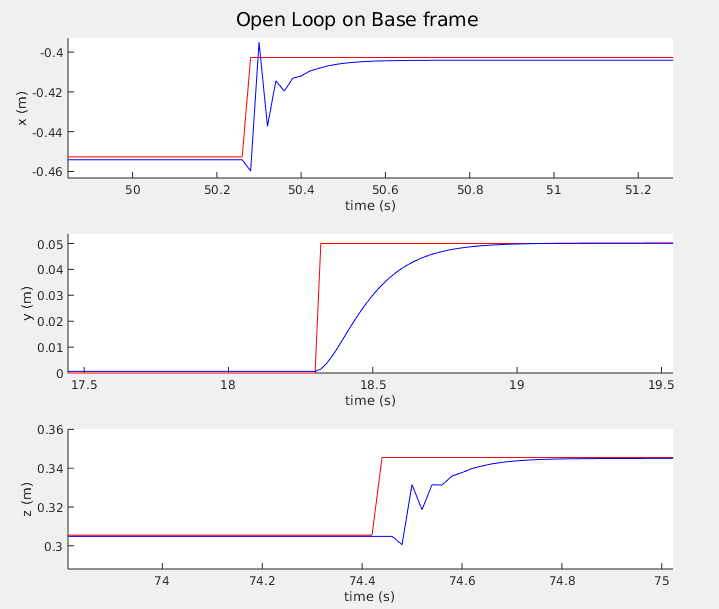
\includegraphics[width=0.8\textwidth]{Images/Section07/openloopBaseFrame.png}
    \caption{Open loop response in base frame for step input}
    \label{fig:OpenLoopGraph}
\end{figure}

\bigbreak
Using the joystick, the user gives an approximate position and corrects the desired position thanks to the camera feedback. As the results show, the open loop is accurate and allows to follow a position. Thus, it was not necessary to set up a closed loop on the real robot. We thus avoided buying a position sensor and saved development and delivery time.

\subsection{Closed loop}

However, we still servoed the robot in position in simulation. To stick to reality, we have modified a bit the robot in simulation compared to the reference robot used. Thus, we were closer to a real case and we were able to test a positional servoing using a proportional integral corrector. All this was done in simulation and was never tested on the real robot because we didn't have the time, we didn't have a sensor and the open loop was enough for a joystick control.
\begin{figure}[H]
    \centering
    \includegraphics[width=0.8\textwidth]{Images/Section07/closedloop\_joystick.png}
    \caption{Closed loop Schema}
    \label{fig:ClosedLoopSchema}
\end{figure}

For the corrector, we have chosen a proportional integral to suppress the error and the possible overshoot. For the adjustment, we did not calculate a theoretical value. We started with a value that works $k_p\less 1$ and $k_i\less 1$ to avoid that the solution diverges. Then we varied the parameters to increase the \gls{tr}\footnote{Also called setting time, it is the time required for the response curve to reach and stay within a range of a certain percentage of the final value} while avoiding oscillations and overshoot. An anti-\gls{windup}\footnote{The situation in a PID feedback controller where a large change in setpoint occurs (say a positive change) and the integral term accumulates a significant error during the rise} was also implemented at the output of the corrector to avoid that the control diverges. Everything was done using python. Even if it is faster to implement the PID using matlab, the deployment on ROS is longer. Thus, python allowed us to test different values for the corrector parameters more quickly. Finally, we subjected the arm to the same step as for the open loop and we obtained the results listed in the table and figure below.
\begin{table}[ht]
    \centering
    \begin{tabular}{|p{1cm} | p{2.3cm} | p{3.5cm} | p{2.3cm}| p{3.3cm} |} 
        \hline
        \textbf{Axis} & \textbf{Step (mm)} &\textbf{Time response (s)} & \textbf{error (mm)} & \textbf{Overshoot (mm)}\\ [0.3ex]
        \hline
        X & 50 & 1.3 & 0 & 0 \\ 
        \hline
        Y & 50 & 1.2 & 0 & 0 \\ 
        \hline
        Z & 50 & 1 & 0 & 0 \\ 
        \hline
    \end{tabular}
    \caption{Closed loop result}
\end{table}
\FloatBarrier

\begin{figure}[H]
    \begin{subfigure}{.5\linewidth}
        \centering
        \includegraphics[width=1\textwidth]{Images/Section07/closedloop\_x.png}
        \caption{X}
        \label{fig:ClosedX}
    \end{subfigure}%
    \begin{subfigure}{.5\linewidth}
        \centering
        \includegraphics[width=1\textwidth]{Images/Section07/closedloop\_y.png}
        \caption{Y}
        \label{fig:ClosedY}
    \end{subfigure}\\[1ex]
    \begin{subfigure}{\linewidth}
        \centering
        \includegraphics[width=0.5\textwidth]{Images/Section07/closedloop\_z.png}
        \caption{Z}
        \label{fig:ClosedZ}
        \end{subfigure}
        \caption{Closed loop response in base frame for step input}
        \label{fig:ClosedLoopGraph}
\end{figure}
\FloatBarrier
As we only realized this part in simulation, we did not really insist on finding the best parameters to optimize the response time. The objective here was rather to set up a closed loop and to show that it works. In view of the results, we can say that it is the case and in the case where we would like to set up a corrector on the real robot, it will be enough to spend time to find the good parameters.

\bigbreak
Finally, we have also studied the behavior of the arm when we control it with the Xbox controller in the camera's frame. We can see that the error when we stop moving the joystick is zero. However, since the response time is higher, the tracking is a little slower.
\begin{figure}[H]
    \begin{subfigure}{.5\linewidth}
        \centering
        \includegraphics[width=1\textwidth]{Images/Section07/xbox\_closed\_x.png}
        \caption{X}
        \label{fig:XboxtrajClosedX}
    \end{subfigure}%
    \begin{subfigure}{.5\linewidth}
        \centering
        \includegraphics[width=1\textwidth]{Images/Section07/xbox\_closed\_y.png}
        \caption{Y}
        \label{fig:XboxtrajClosedY}
    \end{subfigure}\\[1ex]
    \begin{subfigure}{\linewidth}
        \centering
        \includegraphics[width=0.5\textwidth]{Images/Section07/xbox\_closed\_z.png}
        \caption{Z}
        \label{fig:XboxtrajClosedZ}
        \end{subfigure}
        \caption{Measure in base frame for random trajectory with closed loop}
        \label{fig:XboxtrajClosed}
\end{figure}
\FloatBarrier